\documentclass[12pt]{article}
\usepackage[utf8]{inputenc}
\usepackage[T1]{fontenc}
\usepackage{graphicx}
\usepackage{hyperref}
\usepackage{tikz} % Inclusion du package tikz
\usetikzlibrary{positioning, arrows.meta, shapes.geometric}
\title{Cahier des Charges Projet MLOps}
\author{Patricia Wintrebert \\ Mimoune Louarradi}
\date{11/01/2024}
\newcommand{\institution}{DataScientest}

\begin{document}
	
\maketitle

\begin{center}
	\large \textbf{Organisme :} \institution
\end{center}

\newpage

\section{Contexte et Objectifs}

Ce projet s’inscrit dans une démarche d’optimisation de l’organisation des forces de l’ordre de la ville de Chicago, notamment en étant capable de prédire des pics de criminalité. Pour une grande ville comme Chicago, il est pertinent de pouvoir prévenir si cela est possible l’apparition de crimes et de surcroît renforcer les équipes lorsque cela est nécessaire, ce qui améliore les délais d’intervention.

La ville de Chicago souhaite la mise en place d’une application évolutive et qui analyse et prédit les données en temps réel. Cette API lui permettra d’améliorer son organisation, sa prise de décision et à optimiser ses opérations et ses ressources humaines. Pour la réalisation de cette API, la ville met à disposition des ressources, c'est-à-dire un dataset contenant le rapport des crimes survenus dans la ville depuis 2001. Ce dataset est mis à jour régulièrement.

Les utilisateurs principaux sont tous utilisateurs finaux ayant les droits d’accès à l’application (Forces de l’ordre, administration etc.)

L’administration et la maintenance de l’application sera effectuée par l’équipe technique en charge de la ville de Chicago. Ceux-ci auront la responsabilité de maintenir à jour, déployer, surveiller les performances et améliorer si besoin l’API pour assurer son fonctionnement optimal.

L'API sera hébergée sur une infrastructure cloud, assurant ainsi flexibilité, haute disponibilité et adaptabilité en fonction de la demande. Cette configuration cloud favorise également une harmonisation aisée avec les systèmes et services déjà en place.

Pour une interaction directe, les utilisateurs finaux pourront accéder à l'API via une plateforme web dotée d'une interface utilisateur conviviale. Par ailleurs, pour une intégration plus poussée et une automatisation avancée, les développeurs et les administrateurs bénéficieront d'un accès direct à l’API, permettant une synergie fluide avec d'autres outils et processus existants.

Pour faire face à cette problématique, nous envisageons la mise en place d'une API spécifiquement 
conçue pour la prédiction des événements criminels. En exploitant les technologies de pointe et en l'hébergeant sur une infrastructure cloud, nous assurons une solution flexible et hautement disponible. Cette API offrira la capacité de réaliser des prédictions en temps réel en se basant sur des données existantes.

\section{Modèle}

\subsection{Collecte des données}

La collecte des données sur les crimes est organisée de manière, où chaque incident est classifié non seulement par région, mais aussi chronologiquement par mois. Cette approche transforme le nombre de crimes en une série temporelle, permettant ainsi une analyse des tendances et des modèles dans le temps.

\subsection{Types de crime}

\begin{itemize}
    \item DECEPTIVE PRACTICE
    \item OTHER OFFENSE
    \item THEFT
    \item ...
\end{itemize}

\subsection{Type de région}

\begin{itemize}
    \item Rogers Park
    \item West Ridge
    \item Uptown
    \item ...
\end{itemize}

\subsection{Modélisation et Prédiction}

Pour anticiper et comprendre l'évolution future de ces tendances criminelles, nous avons intégré l'utilisation d'un outil analytique et de prédiction des séries temporelles Prophet, accessible via PyPI.
Le package Prophet  intègre et traite les variations saisonnières ainsi que les impacts des jours fériés, ce qui rend ses prédictions particulièrement robustes et fiables. Ces prédictions sont essentielles pour la mise en place d'une stratégie de planification efficace et pour une allocation optimale des ressources dans le cadre de la lutte contre la criminalité.

\subsection{Code et Implémentation}

Le cœur de notre modèle est incarné par la classe \texttt{ChicagoCrimePredictor}, structurée comme suit : \texttt{ChicagoCrimePredictor(months\_pred=12, data\_dir=DATA\_DIR)}.

Cette classe est conçue pour être flexible et adaptative, avec deux arguments principaux lors de l'initialisation :

\begin{itemize}
	\item \texttt{months\_pred}: Cet argument détermine la période de prédiction, permettant aux utilisateurs de spécifier le nombre de mois pour lesquels ils souhaitent obtenir des prévisions.
	\item \texttt{data\_dir}: Il s'agit du répertoire contenant les données brutes, permettant au modèle d'accéder et de traiter l'ensemble des informations nécessaires.
\end{itemize}

\subsection{Exemple d'application}

Dans le cas d'étude présenté, le modèle est entraîné sur les données collectées depuis l'année 2001 jusqu'en décembre 2022. À partir de ces données, des prédictions sont générées pour une durée d'un an, couvrant la période de janvier 2023 à décembre 2023. Cette approche permet non seulement de comprendre les tendances passées mais aussi d'anticiper avec une certaine précision les évolutions futures dans le domaine de la criminalité.

\paragraph{Focus sur la Criminalité dans la Région d'Austin:}
Pour cette étude, nous avons choisi de concentrer nos efforts sur la prédiction des crimes de type “ASSAULT” dans la région spécifique d'Austin. Cette focalisation est guidée par l'importance croissante de comprendre et de prévenir les actes de violence dans cette zone. Notre modèle, grâce à la méthode \texttt{return\_data}, est configurable et peut être adapté selon différents paramètres, notamment:

\begin{itemize}
	\item \texttt{type\_incident} : Permet de spécifier le type de crime à analyser, dans notre cas “ASSAULT”.
	\item \texttt{community\_area} : Cible une région spécifique pour la prédiction, ici la région d'Austin.
\end{itemize}



\subsection{Métriques d’évaluation}

\subsubsection{Mean Absolute Error (MAE)}

\textbf{Formule:} 
\[ MAE = \frac{1}{n} \sum_{i=1}^{n} \left| y_i - \hat{y}_i \right| \]

\textbf{Description :} Le MAE mesure la différence moyenne entre les valeurs observées (réelles) et les valeurs prédites par le modèle. Pour le calculer, on prend la différence absolue (sans tenir compte du signe) entre chaque paire de valeurs observée et prédite, et ensuite on calcule la moyenne de ces différences.

\textbf{Interprétation :} Un MAE plus petit indique une meilleure performance du modèle. C'est une mesure facile à comprendre car elle est exprimée dans les mêmes unités que les données observées. Par contre, comme elle utilise la valeur absolue, elle ne tient pas compte de la direction des erreurs (sous-estimation ou sur-estimation).

\subsubsection{Root Mean Squared Error (RMSE)}

\textbf{Formule:} 
\[ RMSE = \sqrt{\frac{1}{n} \sum_{i=1}^{n} (y_i - \hat{y}_i)^2} \]

\textbf{Description :} Le RMSE est similaire au MAE mais donne plus de poids aux erreurs plus grandes. On calcule d'abord la différence entre chaque valeur observée et prédite, on élève ces différences au carré, puis on en calcule la moyenne. Finalement, on prend la racine carrée de cette moyenne.

\textbf{Interprétation :} Un RMSE plus faible signifie une meilleure précision du modèle. Le RMSE est plus sensible aux erreurs importantes, ce qui peut être un avantage dans certains contextes où ces erreurs sont plus problématiques. Comme le MAE, le RMSE est exprimé dans les mêmes unités que les valeurs observées.

\subsubsection{R2 (Coefficient de détermination)}

\textbf{Formule:} 
\[ R^2 = 1 - \frac{\sum_{i=1}^{n} (y_i - \hat{y}_i)^2}{\sum_{i=1}^{n} (y_i - \bar{y})^2} \]

\textbf{Description :} Le R2 mesure la proportion de la variance des valeurs observées qui est expliquée par le modèle. Il est calculé en comparant la variance des erreurs du modèle avec la variance totale des valeurs observées.

\textbf{Interprétation :} Un R2 proche de 1 indique que le modèle explique une grande partie de la variance des données, tandis qu'un R2 proche de 0 indique que le modèle n'explique pas bien la variance des données. Le R2 est une mesure utile pour comparer différents modèles entre eux, mais il ne doit pas être le seul critère de jugement, surtout si les données ne suivent pas une distribution normale ou si le modèle est complexe.


\subsection{Résultats d’évaluation}

\begin{figure}[htbp]
	\centering
	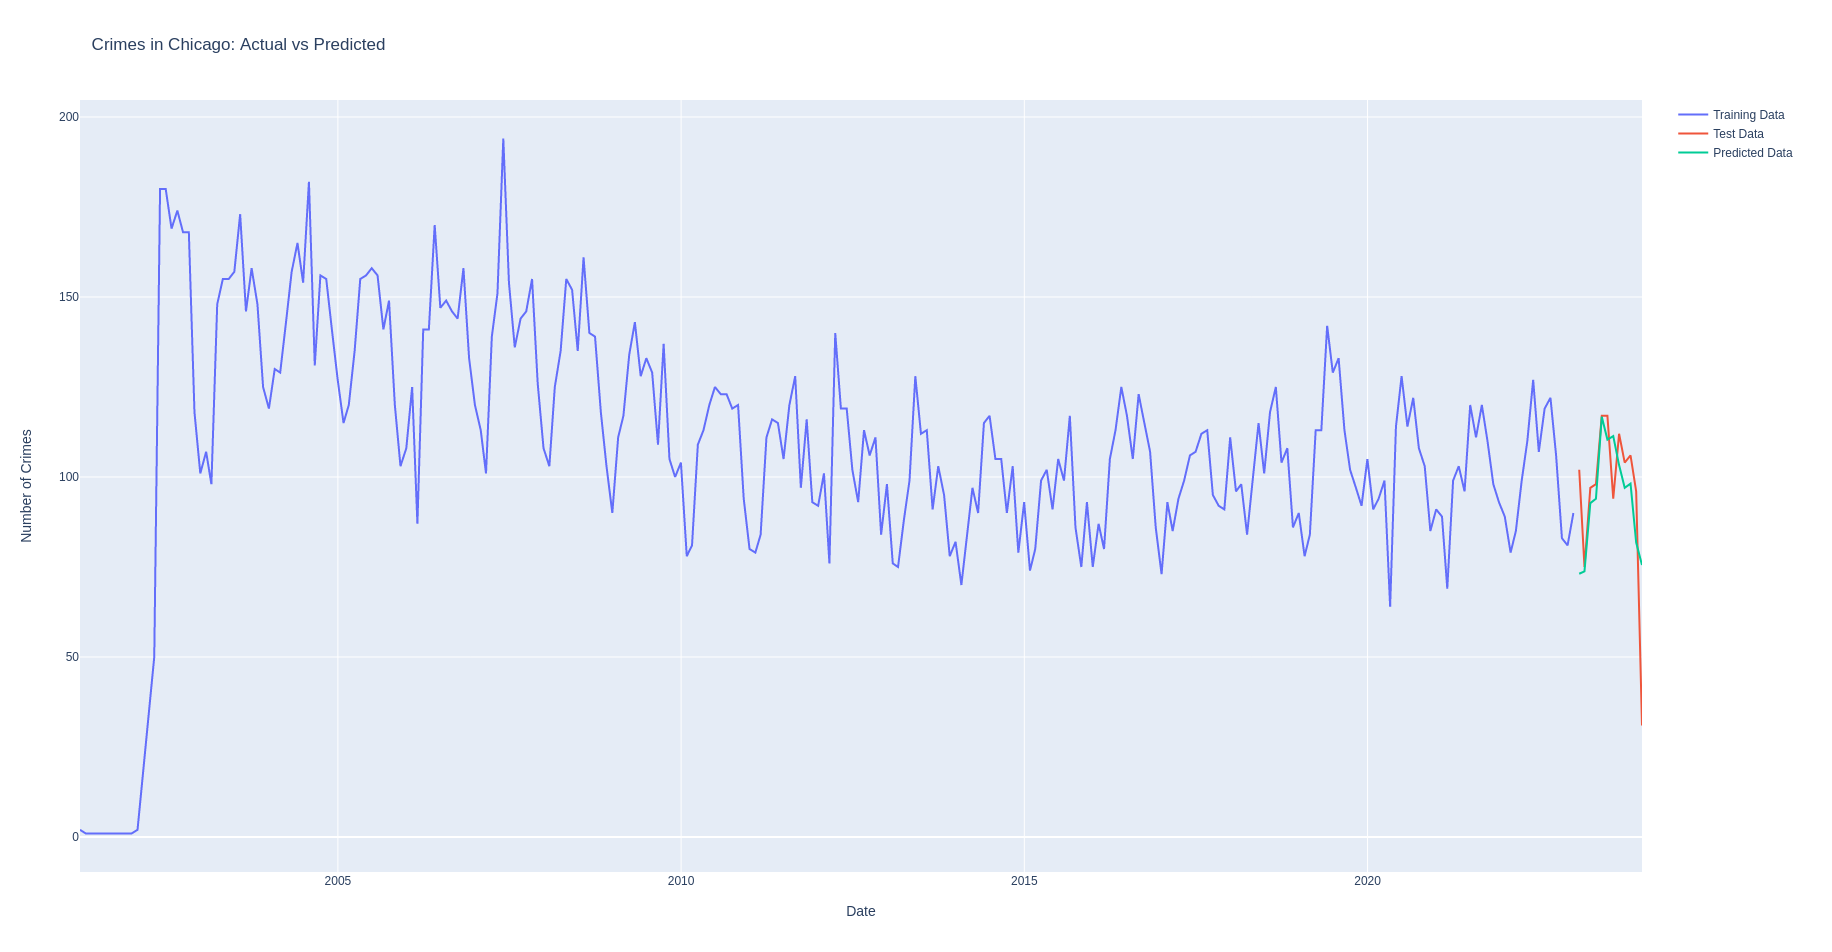
\includegraphics[width=0.7\textwidth]{figure_Assault_Austin.png}
	\caption{Résultats de l'évaluation pour les crimes de type ASSAULT dans la région d'Austin.}
	\label{fig:assault_austin}
\end{figure}

\begin{table}[htbp]
	\centering
	\caption{Métriques du modèle pour les crimes de type ASSAULT dans la région d'Austin}
	\begin{tabular}{|l|c|}
		\hline
		Métrique & Valeur \\
		\hline
		Mean Absolute Error (MAE) & 12.06 \\
		Root Mean Squared Error (RMSE) & 17.28 \\
		R² & 0.4 \\
		\hline
	\end{tabular}
	\label{tab:metrics_assault_austin}
\end{table}
Une base de données SQLite a été créée, permettant ainsi l'enregistrement des métriques pour chaque exécution.
\begin{figure}[htbp]
	\centering
	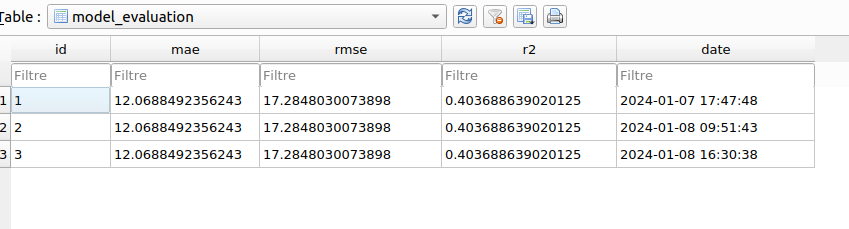
\includegraphics[width=0.7\textwidth]{Capture_Sqlite.png}
	\caption{Résultats de l'évaluation : capture base de donnée Sqlite}
	\label{fig:assault_austin}
\end{figure}




\section{API}

\begin{itemize}
	\item \textbf{Authentification} : Ce point d'accès est crucial pour garantir la sécurité et l'intégrité de l'API. Il permet l'authentification des utilisateurs et administrateurs, en utilisant la méthode d'authentification jetons OAuth. Cette étape assure que seuls les utilisateurs autorisés peuvent accéder aux fonctionnalités de l'API.
	\item \textbf{Prédiction} : Ce endpoint joue un rôle central dans l'application en permettant aux utilisateurs d'obtenir des prédictions sur les crimes. Il utilise des modèles d'apprentissage automatique en tant que séries temporelles et de traitement de données pour analyser et interpréter les tendances des crimes.
	\item \textbf{Evaluation} : Ce point d'accès fournit des métriques essentielles sur la performance du modèle de prédiction. Il offre des statistiques telles que l'Erreur Moyenne Absolue (MAE), l'Erreur Quadratique Moyenne (MSE), et le coefficient de détermination (R2). Ces métriques aident à évaluer l'exactitude et la fiabilité du modèle de prédiction.
	\item \textbf{Réentraînement} : Introduit comme une nouvelle fonctionnalité, ce endpoint permet de réentraîner le modèle de prédiction automatiquement lorsque les métriques de performance tombent en dessous d'un seuil prédéfini. Ce processus assure que le modèle reste performant et précis, en s'adaptant aux nouvelles tendances et données.
	\item \textbf{Mise à jour des données} : Ce point d'accès est essentiel pour maintenir la pertinence du modèle de prédiction. Il permet une mise à jour régulière et automatique des données utilisées par le modèle, en intégrant les dernières informations relatives aux crimes. Cette mise à jour garantit que le modèle reste efficace et adapté à l'évolution constante des schémas de criminalité.
\end{itemize}


\section{Testing \& Monitoring}

Lors de chaque mise à jour de la branche master du repository, un workflow lance automatiquement différents tests :

\begin{enumerate}
	\item \texttt{test\_auth.py}: Les tests de ce script utilisent la bibliothèque TestClient et aident à s'assurer que l'application FastAPI fonctionne correctement en vérifiant diverses fonctionnalités telles que l'authentification, la génération de tokens, la vérification de mots de passe et l'accès aux données sécurisées.
	
	\item \texttt{test\_verify\_password()} : Ce test vérifie la fonction verify\_password en utilisant une comparaison avec des mots de passe hashés. Il vérifie si la fonction verify\_password renvoie True lorsque le mot de passe fourni correspond au mot de passe hashé, et False lorsque le mot de passe fourni est incorrect.
	
	\item \texttt{test\_generate\_token()} : Ce test vérifie la fonction generate\_token. Il génère un token en utilisant un nom d'utilisateur fictif et vérifie si le résultat est une chaîne de caractères non vide (une chaîne de token valide).
	
	\item \texttt{test\_login\_success()} : Ce test vérifie la route /login lorsque la tentative de connexion est réussie. Il envoie une requête POST avec un nom d'utilisateur et un mot de passe valides et vérifie si la réponse renvoie un code de statut HTTP 200 (OK) et si un jeton d'accès (access\_token) est présent dans la réponse JSON.
	
	\item \texttt{test\_login\_failure()} : Ce test vérifie la route /login lorsque la tentative de connexion échoue en envoyant un mot de passe incorrect. Il envoie une requête POST avec un nom d'utilisateur valide mais un mot de passe incorrect, puis vérifie si la réponse renvoie un code de statut HTTP 401 (Unauthorized) et si aucun jeton d'accès n'est présent dans la réponse JSON.
	
	\item \texttt{test\_secure\_data\_with\_token()} : Ce test vérifie la route /secure-data en utilisant un jeton d'accès valide. Il génère un jeton d'accès pour un utilisateur fictif, ajoute ce jeton aux en-têtes de la requête GET, puis vérifie si la réponse renvoie un code de statut HTTP 200 (OK) et si le message dans la réponse JSON indique que les données sont sécurisées pour l'utilisateur spécifié.
	
	\item \texttt{test\_secure\_data\_without\_token()} : Ce test vérifie la route /secure-data sans fournir de jeton d'accès. Il envoie une requête GET sans jeton d'accès dans les en-têtes et vérifie si la réponse renvoie un code de statut HTTP 401 (Unauthorized), ce qui signifie que l'accès aux données sécurisées est refusé en l'absence de jeton d'accès.
	
	\item \texttt{test.bdd.py} : Ce test utilise la bibliothèque requests pour effectuer une requête GET vers une URL spécifique et vérifier si l'API répond correctement:
	\begin{itemize}
		\item \texttt{test\_api\_url()} : Ce test vise à vérifier si l'URL de l'API réagit correctement. Il crée une variable url contenant l'URL de l'API cible, qui est "https://data.cityofchicago.org/resource/ijzp-q8t2.json" dans ce cas. Ensuite, il envoie une requête GET à l'URL à l'aide de requests.get(url). Le test vérifie ensuite si la réponse de la requête renvoie un code de statut HTTP 200 (OK) en utilisant l'assertion assert response.status\_code == 200.
	\end{itemize}
	
	\item \texttt{test\_chicago\_crime\_predictor.py} : Ce script contient une série de tests unitaires pour la classe ChicagoCrimePredictor, qui est une classe utilisée pour prédire les taux de criminalité à Chicago:
	\begin{itemize}
		\item \texttt{test\_init()}: Ce test vérifie le constructeur de la classe ChicagoCrimePredictor. Il crée une instance de ChicagoCrimePredictor avec des paramètres spécifiques (6 mois de prévision et un répertoire de données 'data') et vérifie que les attributs de l'instance sont corrects, notamment \_month\_pred est égal à 6, data\_dir est un objet Path pointant vers 'data', et que l'attribut model est initialisé à None.
		
		\item \texttt{@fixture mock\_df\_crime} et \texttt{@fixture mock\_df\_socio}: Ces décorateurs de fixture définissent deux DataFrames fictifs (mock\_df\_crime et mock\_df\_socio) qui serviront de données simulées pour les tests.
		
		\item \texttt{test\_load\_df\_crimes()}: Ce test vérifie la méthode load\_df\_crimes() de la classe ChicagoCrimePredictor. Il utilise mocker.patch pour simuler l'appel à pandas.read\_csv et vérifie que la méthode retourne un DataFrame qui correspond à mock\_df\_crime.
		
		\item \texttt{test\_load\_df\_socio()}: Ce test vérifie la méthode load\_df\_socio() de la classe ChicagoCrimePredictor. Il utilise également mocker.patch pour simuler l'appel à pandas.read\_csv et vérifie que la méthode retourne un DataFrame qui correspond à mock\_df\_socio.
		
		\item \texttt{test\_return\_data()}: Ce test vérifie la méthode return\_data() de la classe ChicagoCrimePredictor. Il utilise des simulations pour charger des DataFrames factices et appelle ensuite la méthode pour obtenir les données d'entraînement et de test. Il vérifie que les données retournées sont des objets DataFrame.
		
		\item \texttt{test\_model\_train()}: Ce test vérifie la méthode model\_train() de la classe ChicagoCrimePredictor. Il utilise mocker.patch pour simuler l'appel à la méthode fit de la classe Prophet (un modèle de séries temporelles) et vérifie que la méthode model\_train() attribue un modèle Prophet à l'instance de predictor.
		
		\item \texttt{test\_model\_predict()}: Ce test vérifie la méthode model\_predict() de la classe ChicagoCrimePredictor. Il simule l'utilisation d'un modèle pré-entraîné, charge ce modèle, attribue le modèle à l'instance de predictor et vérifie que la méthode model\_predict() renvoie des prédictions non vides.
	\end{itemize}
\end{enumerate}


\section{Schéma d’implémentation}
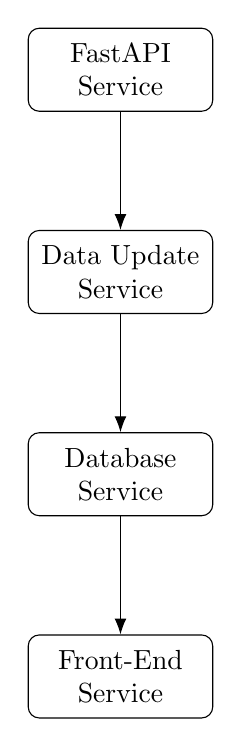
\begin{tikzpicture}[
node distance=1.5cm,
auto,
block/.style={
	rectangle,
	draw,
	text width=6em,
	align=center,
	rounded corners,
	minimum height=3em
},
line/.style={
	draw, -{Latex[length=2mm]}
}
]

% Nodes
\node[block] (fastapi) {FastAPI Service};
\node[block, below=of fastapi] (dataupdate) {Data Update Service};
\node[block, below=of dataupdate] (database) {Database Service};
\node[block, below=of database] (frontend) {Front-End Service};

% Lines
\draw[line] (fastapi) -- (dataupdate);
\draw[line] (dataupdate) -- (database);
\draw[line] (database) -- (frontend);

\end{tikzpicture}


\end{document}
